%==============================================================================
% BuildStream: A Reproducible AWS-Native Reference Architecture for Mobile CI/CD
% with Ephemeral Code-Signing Credentials
%
% Preprint (not peer reviewed). Prepared for arXiv submission.
%==============================================================================
\documentclass[conference]{IEEEtran}
\IEEEoverridecommandlockouts

\usepackage{cite}
\usepackage{amsmath,amssymb,amsfonts}
\usepackage{graphicx}
\usepackage{xcolor}
\usepackage{booktabs}
\usepackage{listings}
\usepackage{float}
\usepackage{url}
\usepackage[hidelinks]{hyperref}
\usepackage{tikz}
\usetikzlibrary{positioning,arrows.meta,fit,backgrounds,calc}
\usepackage[T1]{fontenc}

% --- Listing style for code (Groovy / shell) -------------------------------
\definecolor{codegray}{gray}{0.95}
\definecolor{codecomment}{rgb}{0.30,0.45,0.30}
\definecolor{codekw}{rgb}{0.10,0.10,0.55}
\lstdefinestyle{bs}{
  backgroundcolor=\color{codegray},
  basicstyle=\ttfamily\scriptsize,
  commentstyle=\color{codecomment}\itshape,
  keywordstyle=\color{codekw}\bfseries,
  breaklines=true,
  captionpos=b,
  showstringspaces=false,
  columns=fullflexible,
  keepspaces=true,
  frame=single,
  framesep=3pt,
  xleftmargin=4pt,
  aboveskip=4pt,
  belowskip=2pt,
  morekeywords={def,pipeline,agent,stages,stage,steps,script,when,post,always,if,else,environment,options,new,return,error}
}
\lstset{style=bs}

\begin{document}

\title{BuildStream: A Reproducible AWS-Native Reference\\ Architecture for Mobile CI/CD with Ephemeral\\ Code-Signing Credentials}

\author{
\IEEEauthorblockN{Santosh Kumar Puppala}
\IEEEauthorblockA{\textit{Independent Researcher}\\
Pennsylvania, USA\\
puppalas97@gmail.com}
}

\maketitle

\begin{abstract}
Mobile application delivery imposes security and operational burdens that web
deployment does not: iOS builds require macOS hardware, code signing depends on
long-lived secret material (Apple \texttt{.p12} certificates and Android
keystores), and distribution spans multiple gated app stores. Common practice
either stores signing credentials on persistent build machines or entrusts them
to third-party hosted continuous-integration (CI) services, both of which widen
the exposure surface for the most sensitive assets in the mobile software supply
chain. We present \emph{BuildStream}, an open-source, AWS-native reference
architecture for mobile CI/CD that keeps signing credentials inside the
organization's own cloud account and reduces their on-disk lifetime to the
duration of a single signing operation. Its central mechanism is a
\emph{pull--use--destroy} ephemeral-credential pattern: signing material is
retrieved from AWS Secrets Manager at sign time, used to sign exactly one
artifact, and erased---together with any transient keychain---before the
workspace is purged. A Jenkins shared-library design routes iOS and Android
builds through a common pipeline that an application adopts with a three-line
configuration. We describe the threat model, the architecture across its
networking, orchestration, build, secrets, artifact, and monitoring layers, and
the signing flows for both platforms. We report a working deployment on Amazon
EC2---including an EC2 Mac Dedicated Host---with end-to-end iOS and Android
pipeline runs, versioned artifacts in S3, and CloudWatch monitoring, and we
analyze the resulting credential-exposure window. We discuss portability to
Bitbucket and IBM UrbanCode Deploy, and we are explicit about the limitations
of the present prototype.
\end{abstract}

\begin{IEEEkeywords}
mobile CI/CD, code signing, secret management, DevSecOps, cloud infrastructure,
ephemeral credentials, least privilege, AWS.
\end{IEEEkeywords}

%==============================================================================
\section{Introduction}
%==============================================================================
Continuous integration and continuous delivery (CI/CD) for mobile applications
is materially harder than for web services. Building an iOS application requires
Apple's toolchain on macOS hardware; building Android requires a specific SDK
and Gradle toolchain; and \emph{both} platforms gate release artifacts behind
mandatory code signing. Signing in turn depends on long-lived secret material:
an Apple distribution certificate exported as a PKCS\#12 (\texttt{.p12}) bundle
together with a provisioning profile for iOS, and a Java KeyStore
(\texttt{.jks}) for Android. These keys are among the most sensitive assets an
organization holds. On Android in particular, the signing key is bound
permanently to an application's package identity: losing or rotating it severs
the ability to ship updates to the existing install base~\cite{androidsign}.

Two operational patterns dominate in practice, and each enlarges the attack
surface around exactly these assets. In the first, an organization runs
persistent build servers and stores certificates and keystores on disk so that
builds can find them. The credential then lives on the machine indefinitely,
readable by any process that compromises the build environment, and its blast
radius spans every build the server ever runs. In the second, the organization
adopts a third-party hosted CI service and uploads its signing credentials to
that vendor. Convenience improves, but the most sensitive secrets in the mobile
supply chain now leave the organization's own trust boundary, and regulated
sectors (finance, healthcare, government) frequently cannot accept that
custody transfer at all.

\textbf{Position.} We argue that mobile signing credentials should (i) never
leave the organization's own cloud account and (ii) exist on a build agent only
for the few seconds in which a signature is actually produced. BuildStream is a
concrete, open-source instantiation of that position on Amazon Web Services
(AWS).

\textbf{Contributions.} This paper makes the following contributions:
\begin{enumerate}
  \item A \emph{pull--use--destroy} ephemeral-credential pattern for mobile code
  signing, instantiated for both Apple \texttt{.p12} signing (via a temporary,
  immediately-destroyed keychain) and Android keystore signing (via a transient
  decoded \texttt{.jks}), with build-log hygiene to prevent secret leakage
  (Section~\ref{sec:ephemeral}).
  \item A complete AWS-native reference architecture that keeps credentials
  in-account, isolates build agents in a private network, and enforces
  least-privilege IAM scoping per secret namespace
  (Section~\ref{sec:arch}).
  \item A Jenkins shared-library implementation that provides zero-configuration,
  three-line onboarding for any mobile application while centralizing all
  pipeline logic at a single point of maintenance
  (Section~\ref{sec:impl}).
  \item An open-source reference implementation and a working-deployment
  evaluation on real AWS infrastructure, including measured credential-exposure
  windows for both platforms (Section~\ref{sec:eval}).
\end{enumerate}

We are deliberately explicit about scope. BuildStream is a \emph{reference
architecture and prototype}, not a peer-reviewed production study. Our
evaluation demonstrates architectural viability and a quantifiable reduction in
credential exposure; it is not a statistical performance benchmark and does not
claim production adoption. Section~\ref{sec:limits} states precisely what is and
is not demonstrated. All code and documentation are publicly
available.\footnote{\url{https://github.com/Santoshkumarpuppala/BuildStream}}

%==============================================================================
\section{Background and Related Work}\label{sec:background}
%==============================================================================
\subsection{Mobile Code Signing}
Apple requires every distributed iOS binary to be signed with a certificate
issued by an enrolled developer account and paired with a provisioning profile
that authorizes specific devices or distribution channels~\cite{applesign}. The
private key and certificate are typically managed as a \texttt{.p12} bundle and
imported into a macOS keychain so that \texttt{xcodebuild} can sign during
export. Android requires that every APK or App Bundle (AAB) be signed with a key
held in a Java KeyStore; the platform pins an application's package name to its
signing key for the lifetime of the app~\cite{androidsign}. Google Play App
Signing optionally lets Google hold the distribution key while the developer
retains an ``upload key,'' but the developer-side signing step is unchanged.
These mechanisms make the signing key a long-lived, high-value, and---on
Android---effectively irreplaceable secret.

\subsection{Secret Management and Just-in-Time Credentials}
The principle of least privilege~\cite{saltzer} argues that a component should
hold only the authority it needs, for only as long as it needs it. Modern secret
managers operationalize this for credentials: AWS Secrets
Manager~\cite{awssm} and HashiCorp Vault~\cite{vault} centralize secret storage
behind access policies and audit logging, and Vault popularized \emph{dynamic}
or short-lived secrets that are issued on demand and expire. National guidance on
secure software supply chains, including the NIST Secure Software Development
Framework~\cite{nistssdf}, similarly emphasizes protecting and minimizing
exposure of signing material. BuildStream applies the just-in-time idea to a
domain where the secret itself cannot be made short-lived---an Android signing
key must persist for years---by instead minimizing the \emph{on-agent lifetime}
of a copy of that secret.

\subsection{CI/CD for Mobile}
Jenkins~\cite{jenkins} is a widely deployed self-hosted automation server whose
shared-library mechanism allows pipeline logic to be centralized and reused
across repositories. Fastlane~\cite{fastlane} provides higher-level actions for
iOS and Android build, signing, and store submission. Hosted services such as
Bitrise, CircleCI, and GitHub Actions~\cite{ghactions} reduce operational effort
but require the organization to store signing credentials within the vendor's
platform and offer limited control over the build environment---particularly for
macOS, where access to dedicated Apple hardware is constrained. AWS offers EC2
Mac Dedicated Hosts that satisfy Apple's macOS licensing terms and allow iOS
builds to run on instances inside the customer's own account and
network~\cite{ec2mac}. BuildStream combines self-hosted Jenkins, Fastlane, and
EC2 Mac with AWS-native secret and artifact services so that the entire signing
path---hardware, credentials, and artifacts---remains within a single AWS
account boundary.

%==============================================================================
\section{Threat Model and Design Goals}\label{sec:threat}
%==============================================================================
\textbf{Assets.} The primary protected assets are the signing credentials
(Apple \texttt{.p12} certificate and password, provisioning profile, Android
keystore and its passwords). Secondary assets are application source code and
build artifacts.

\textbf{Adversaries and assumptions.} We assume the AWS control plane and the
Jenkins controller are trusted. We treat build agents as \emph{semi-trusted}:
an agent is correctly provisioned but a build job could be subverted at
runtime---for example by a malicious dependency or a compromised build
script---and could attempt to read whatever credential material is present on
disk or in the build log. We also consider a network adversary attempting to
reach agents directly, and a low-privilege insider holding scoped IAM
credentials. We do not defend against a full compromise of the AWS account root
or of the Jenkins controller host.

\textbf{Design goals.} From this model we derive:
\begin{itemize}
  \item[\textbf{G1}] \emph{No persistence}: signing credentials never remain on a
  build agent between builds.
  \item[\textbf{G2}] \emph{In-account custody}: credentials never leave the
  organization's AWS account.
  \item[\textbf{G3}] \emph{Least privilege}: an agent can read only the secret
  namespace and artifact bucket it requires.
  \item[\textbf{G4}] \emph{Network isolation}: build agents accept no inbound
  traffic except from the controller.
  \item[\textbf{G5}] \emph{Log hygiene}: secret values never appear in build
  logs.
  \item[\textbf{G6}] \emph{Low onboarding cost}: adopting the pipeline requires
  minimal per-application configuration.
  \item[\textbf{G7}] \emph{Auditability}: build and access events are centrally
  logged.
\end{itemize}

%==============================================================================
\section{System Architecture}\label{sec:arch}
%==============================================================================
BuildStream is organized into six layers, summarized in
Table~\ref{tab:layers} and depicted in Fig.~\ref{fig:arch}.

\begin{table}[t]
\caption{Architectural layers and the goals they address.}
\label{tab:layers}
\centering
\footnotesize
\begin{tabular}{@{}p{1.55cm}p{4.0cm}p{1.4cm}@{}}
\toprule
\textbf{Layer} & \textbf{Components} & \textbf{Goals} \\
\midrule
Source control & GitHub repositories, webhooks & G6, G7 \\
Orchestration & Jenkins controller (EC2, public subnet); \texttt{mobile-lib} shared library & G6 \\
Build & EC2 Mac Dedicated Host (private subnet); Xcode, Gradle, Fastlane & G1, G4 \\
Secrets & AWS Secrets Manager; scoped IAM roles & G2, G3 \\
Artifacts & Amazon S3 (versioned bucket) & G3, G7 \\
Monitoring & CloudWatch agent, alarms, SNS & G7 \\
\bottomrule
\end{tabular}
\end{table}

\begin{figure*}[t]
\centering
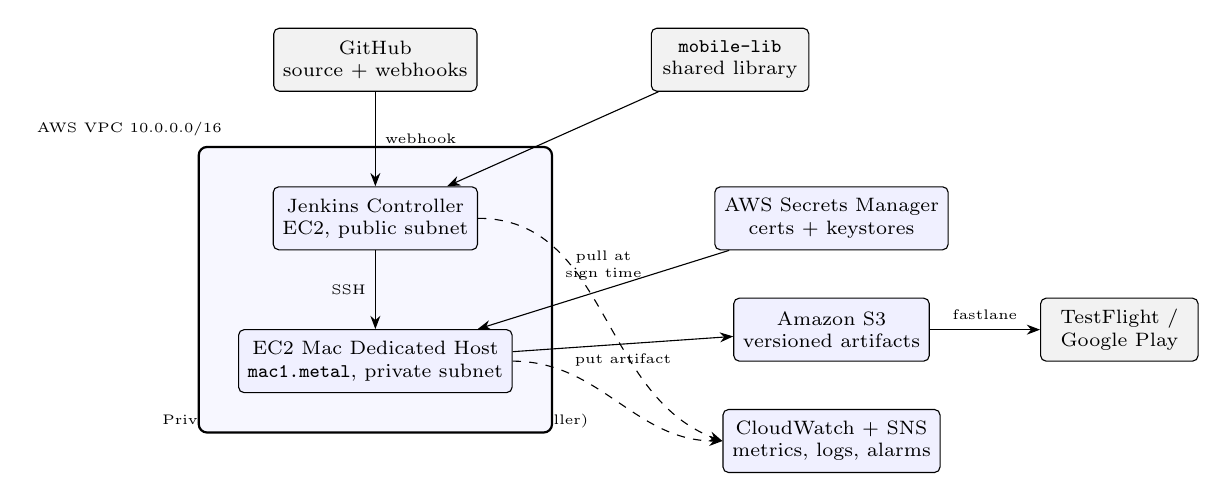
\begin{tikzpicture}[
  font=\scriptsize,
  box/.style={draw,rounded corners=2pt,align=center,minimum height=8mm,minimum width=20mm,fill=white},
  svc/.style={box,fill=blue!6},
  ext/.style={box,fill=gray!10},
  >={Stealth[]},
]
% external source
\node[ext] (gh) {GitHub\\source + webhooks};
\node[ext,right=22mm of gh] (lib) {\texttt{mobile-lib}\\shared library};

% VPC contents
\node[svc,below=12mm of gh] (jenkins) {Jenkins Controller\\EC2, public subnet};
\node[svc,below=10mm of jenkins] (mac) {EC2 Mac Dedicated Host\\\texttt{mac1.metal}, private subnet};

% subnet frames
\begin{scope}[on background layer]
  \node[draw,dashed,fit=(jenkins),inner sep=4pt,label={[font=\tiny]above:Public subnet}] (pub) {};
  \node[draw,dashed,fit=(mac),inner sep=4pt,label={[font=\tiny]below:Private subnet (no inbound except from controller)}] (priv) {};
  \node[draw,thick,rounded corners=3pt,fill=blue!3,fit=(pub)(priv),inner sep=10pt,label={[font=\tiny]above left:AWS VPC 10.0.0.0/16}] (vpc) {};
\end{scope}

% right-hand services
\node[svc,right=30mm of jenkins] (sm) {AWS Secrets Manager\\certs + keystores};
\node[svc,below=6mm of sm] (s3) {Amazon S3\\versioned artifacts};
\node[svc,below=6mm of s3] (cw) {CloudWatch + SNS\\metrics, logs, alarms};

% distribution
\node[ext,right=14mm of s3] (store) {TestFlight /\\Google Play};

% edges
\draw[->] (gh) -- node[right,font=\tiny]{webhook} (jenkins);
\draw[->] (lib) -- (jenkins);
\draw[->] (jenkins) -- node[left,font=\tiny]{SSH} (mac);
\draw[->] (sm) -- node[above,font=\tiny,align=center]{pull at\\sign time} (mac);
\draw[->] (mac) -- node[below,font=\tiny]{put artifact} (s3);
\draw[->] (s3) -- node[above,font=\tiny]{fastlane} (store);
\draw[->,dashed] (mac.east) to[out=0,in=180] (cw.west);
\draw[->,dashed] (jenkins.east) to[out=0,in=160] (cw.west);
\end{tikzpicture}
\caption{BuildStream reference architecture. Build agents run in a private
subnet that accepts inbound connections only from the Jenkins controller.
Signing credentials are pulled from Secrets Manager directly onto the agent at
sign time and never traverse the controller. Signed artifacts are written to a
versioned S3 bucket; distribution to TestFlight or Google Play occurs only on
the \texttt{main} branch.}
\label{fig:arch}
\end{figure*}

\subsection{Network Isolation (G4)}
The deployment provisions a Virtual Private Cloud (VPC) with a public subnet for
the Jenkins controller and a private subnet for the Mac build agents. The
agents' security group permits inbound SSH only from the controller's security
group; they expose no public interface. The controller, reachable by
administrators on its web port, dispatches jobs to agents over SSH.

\subsection{Least-Privilege IAM (G3)}
The controller and the agents assume distinct IAM roles. The policy attached to
build infrastructure scopes Secrets Manager access to two namespaces,
\texttt{ios/*} and \texttt{android/*}, and scopes S3 access to a single artifact
bucket. An agent therefore cannot read secrets outside the mobile-signing
namespaces, nor write to any other bucket. Listing~\ref{lst:iam} shows the core
of the policy.

\begin{lstlisting}[language=,caption={Least-privilege policy fragment scoping secret and artifact access.},label={lst:iam}]
{ "Effect": "Allow",
  "Action": ["secretsmanager:GetSecretValue"],
  "Resource": [
    "arn:aws:secretsmanager:us-east-1:*:secret:ios/*",
    "arn:aws:secretsmanager:us-east-1:*:secret:android/*" ] },
{ "Effect": "Allow",
  "Action": ["s3:PutObject","s3:GetObject","s3:ListBucket"],
  "Resource": [
    "arn:aws:s3:::myhub-mobile-artifacts",
    "arn:aws:s3:::myhub-mobile-artifacts/*" ] }
\end{lstlisting}

\subsection{Versioned Artifact Storage (G7)}
Signed artifacts are written to a versioned S3 bucket under a structured key that
encodes platform, application, branch, and build number:
\begin{center}
\texttt{<platform>/<app>/<branch>/<build>/<app>.<ext>}
\end{center}
This scheme makes every build independently addressable, supports per-branch
retention via S3 lifecycle rules, and provides an audit trail linking each
artifact to the commit and build that produced it.

%==============================================================================
\section{The Ephemeral Credential Pattern}\label{sec:ephemeral}
%==============================================================================
The core security mechanism of BuildStream is a \emph{pull--use--destroy}
discipline applied uniformly to signing material:

\begin{enumerate}
  \item \textbf{Pull.} At the start of the signing stage, the agent retrieves the
  required secrets from Secrets Manager using its scoped IAM role.
  \item \textbf{Use.} The decoded material is used to sign exactly one artifact.
  \item \textbf{Destroy.} Every transient artifact---the decoded key file and any
  keychain created to hold it---is deleted immediately after signing, and the
  entire workspace is purged at the end of the build.
\end{enumerate}

Figure~\ref{fig:window} situates the resulting exposure window within the
pipeline: a decoded copy of the signing key exists on the agent only during the
\emph{Sign} stage, which in our measurements lasts a few seconds
(Section~\ref{sec:eval}), in contrast to the indefinite on-disk lifetime of the
persistent-server baseline.

\begin{figure}[t]
\centering
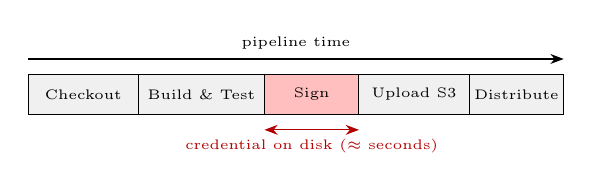
\begin{tikzpicture}[font=\scriptsize,>={Stealth[]}]
\def\h{5mm}
\foreach \x/\w/\name/\col in {0/14/Checkout/gray!12, 14/16/Build \& Test/gray!12, 30/12/Sign/red!25, 42/14/Upload S3/gray!12, 56/12/Distribute/gray!12} {
  \draw[fill=\col] (\x mm,0) rectangle ++(\w mm,\h);
  \node[font=\tiny] at (\x mm+\w mm/2, \h/2) {\name};
}
\draw[<->,red!70!black] (30mm,-2mm) -- node[below,font=\tiny,red!70!black]{credential on disk ($\approx$ seconds)} (42mm,-2mm);
\draw[->] (0,\h+2mm) -- node[above,font=\tiny]{pipeline time} (68mm,\h+2mm);
\end{tikzpicture}
\caption{Credential-exposure window. A decoded signing key exists on the agent
only during the Sign stage; it is erased before Upload, and the workspace is
purged after Distribute.}
\label{fig:window}
\end{figure}

\subsection{Android Signing}
The Android signing routine pulls the keystore and its passwords through a small
helper that extracts named fields from each JSON secret, decodes the keystore to
a temporary \texttt{.jks}, invokes \texttt{jarsigner}, and then removes the
keystore. Shell tracing is disabled (\texttt{set +x}) so that passwords never
reach the build log (G5). Listing~\ref{lst:androidsign} reproduces the
implementation.

\begin{lstlisting}[language=Java,caption={Android pull--use--destroy signing (Groovy).},label={lst:androidsign}]
def sign(String appName) {
  def aws = new AwsSecrets(script)
  def ksB64 = aws.getSecretField('android/keystore','keystore')
  def ksPwd = aws.getSecretField('android/keystore-password','password')
  def alias = aws.getSecretField('android/key-alias','alias')
  def keyPwd= aws.getSecretField('android/key-password','password')
  script.sh """
    set +x   # suppress trace: no passwords in build log
    echo '${ksB64}' | base64 -d > keystore.jks
    AAB=\$(find . -name "*.aab" | head -1)
    jarsigner -sigalg SHA256withRSA -digestalg SHA-256 \
      -keystore keystore.jks -storepass '${ksPwd}' \
      -keypass '${keyPwd}' "\$AAB" '${alias}'
    mkdir -p output && cp "\$AAB" output/${appName}.aab
    rm -f keystore.jks    # destroy ephemeral credential
  """
}
\end{lstlisting}

\subsection{iOS Signing}
The iOS production signing path follows the same discipline using a
\emph{temporary keychain}. The \texttt{.p12} certificate and its password are
pulled and decoded; a dedicated keychain is created with
\texttt{security create-keychain}; the certificate is imported; the archive is
exported and signed with \texttt{xcodebuild -exportArchive}; and the keychain is
then destroyed with \texttt{security delete-keychain}, followed by removal of the
decoded certificate file. The keychain exists only for the duration of the
export and is never added to the agent's login keychain, so no signing identity
persists.

\subsection{Defense-in-Depth Summary}
The pattern jointly satisfies G1, G2, and G5: credentials are fetched in-account
under a scoped role (G2/G3), exist on disk only transiently and are explicitly
destroyed (G1), and are kept out of logs by disabling shell tracing around their
use (G5). The end-of-build workspace purge (\texttt{cleanWs}) provides a
belt-and-suspenders guarantee that nothing survives the build.

%==============================================================================
\section{Implementation}\label{sec:impl}
%==============================================================================
BuildStream's pipeline logic is packaged as a Jenkins shared library,
\texttt{mobile-lib}, comprising a global pipeline function and a small set of
per-concern classes (an AWS secrets helper, an iOS pipeline, an Android pipeline,
and a notifier). Centralizing the logic means an improvement deploys to every
application at once and no application repository contains pipeline code beyond a
three-line declaration (Listing~\ref{lst:jenkinsfile}), satisfying G6.

\begin{lstlisting}[language=Java,caption={Complete CI/CD integration for an application.},label={lst:jenkinsfile}]
@Library('mobile-lib') _
mobilePipeline(platform: 'ios', appName: 'MyHub')
\end{lstlisting}

\subsection{Platform Routing}
A single entry point, \texttt{mobilePipeline}, derives the triggering branch,
validates the requested platform, and dispatches each stage to the appropriate
platform class. Distribution is gated on the \texttt{main} branch so that feature
branches build and test without signing or publishing. Listing~\ref{lst:route}
shows the routing skeleton.

\begin{lstlisting}[language=Java,caption={Platform routing and branch gating (abridged).},label={lst:route}]
def call(Map config = [:]) {
  def platform = config.platform?.toLowerCase()
  def appName  = config.appName ?: 'UnknownApp'
  def branch   = env.BRANCH_NAME ?: 'main'
  def isMain   = (branch == 'main')
  if (!platform) error "platform required: 'ios' or 'android'"
  pipeline {
    agent { label 'mac-agent' }
    options { disableConcurrentBuilds(); timeout(time:60,unit:'MINUTES') }
    stages {
      stage('Build & Test') { steps { script {
        if (platform=='ios') new IosPipeline(this).buildAndTest(appName)
        else                 new AndroidPipeline(this).buildAndTest(appName)
      }}}
      stage('Sign')         { /* platform sign() */ }
      stage('Upload to S3') { /* structured key */ }
      stage('Distribute')   { when { expression { isMain } } }
    }
    post { always { script { /* notify */ }; cleanWs() } }
  }
}
\end{lstlisting}

\subsection{Operational Concerns}
The pipeline disables concurrent builds to guarantee workspace isolation, sets a
build timeout, and rotates build history. A notifier reports the final result
(and is wired for Slack delivery). The same library serves both reference
applications used in our evaluation, \texttt{myhub-ios} and
\texttt{myhub-android}, unchanged.

%==============================================================================
\section{Evaluation}\label{sec:eval}
%==============================================================================
We deployed BuildStream on a real AWS account in \texttt{us-east-1}: a Jenkins
controller on EC2, an EC2 Mac Dedicated Host registered as the build agent
(\texttt{mac-mini-agent}), Secrets Manager entries for the iOS and Android
signing material, a versioned S3 bucket, and the CloudWatch agent on the build
host. We then exercised the pipeline end to end for both platforms. Our
evaluation answers three questions: (Q1) does the architecture function end to
end on real infrastructure? (Q2) what credential-exposure window does the
ephemeral pattern actually yield? (Q3) what is the onboarding cost?

\subsection{Q1: End-to-End Functionality}
A library-load job confirmed that \texttt{mobile-lib} loads and exposes the
pipeline entry point. A verification job confirmed that the agent has the
required toolchain and---using only its scoped IAM role---can enumerate the
expected secrets (\texttt{ios/apple-p12-cert}, \texttt{ios/apple-p12-password},
\texttt{android/keystore}); see Fig.~\ref{fig:secrets}. Full pipeline runs then
completed all stages for both platforms (Fig.~\ref{fig:pipelines}), producing
signed artifacts at the expected versioned S3 keys
(Fig.~\ref{fig:s3}): \texttt{ios/MyHub/main/17/MyHub.ipa} (5.4\,MB) and
\texttt{android/MyHub/main/5/MyHub.aab} (20.7\,MB).

\begin{figure}[t]
\centering
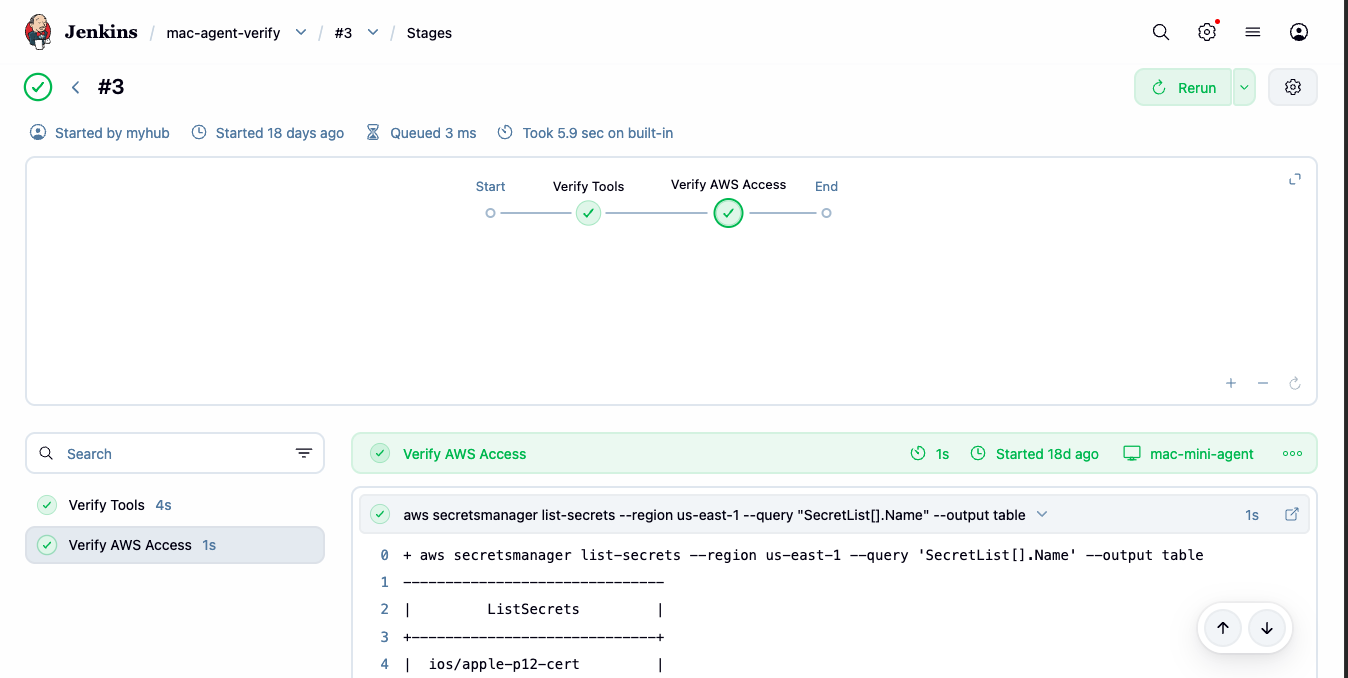
\includegraphics[width=\columnwidth]{figures/jenkins-aws-secrets-verified.png}
\caption{Agent-side verification: using only its scoped instance role, the build
agent enumerates the mobile-signing secrets via the Secrets Manager API.}
\label{fig:secrets}
\end{figure}

\begin{figure}[t]
\centering
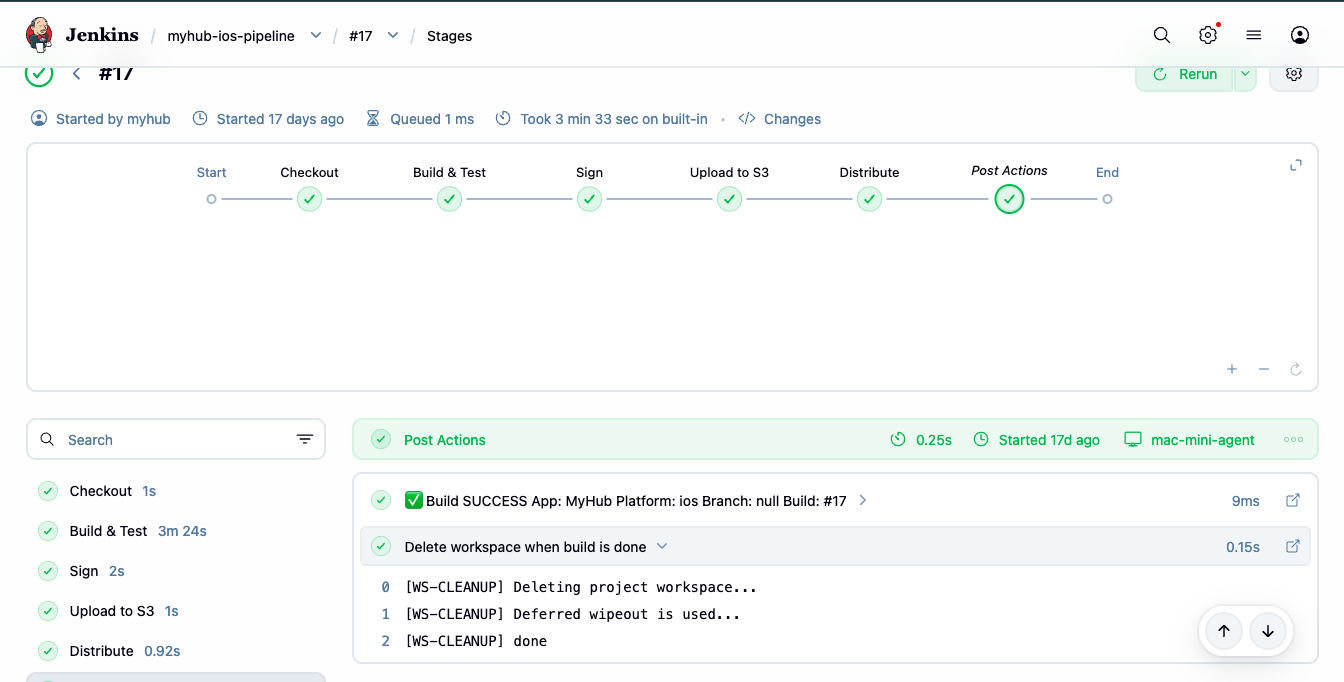
\includegraphics[width=\columnwidth]{figures/jenkins-ios-pipeline-success.png}\\[2pt]
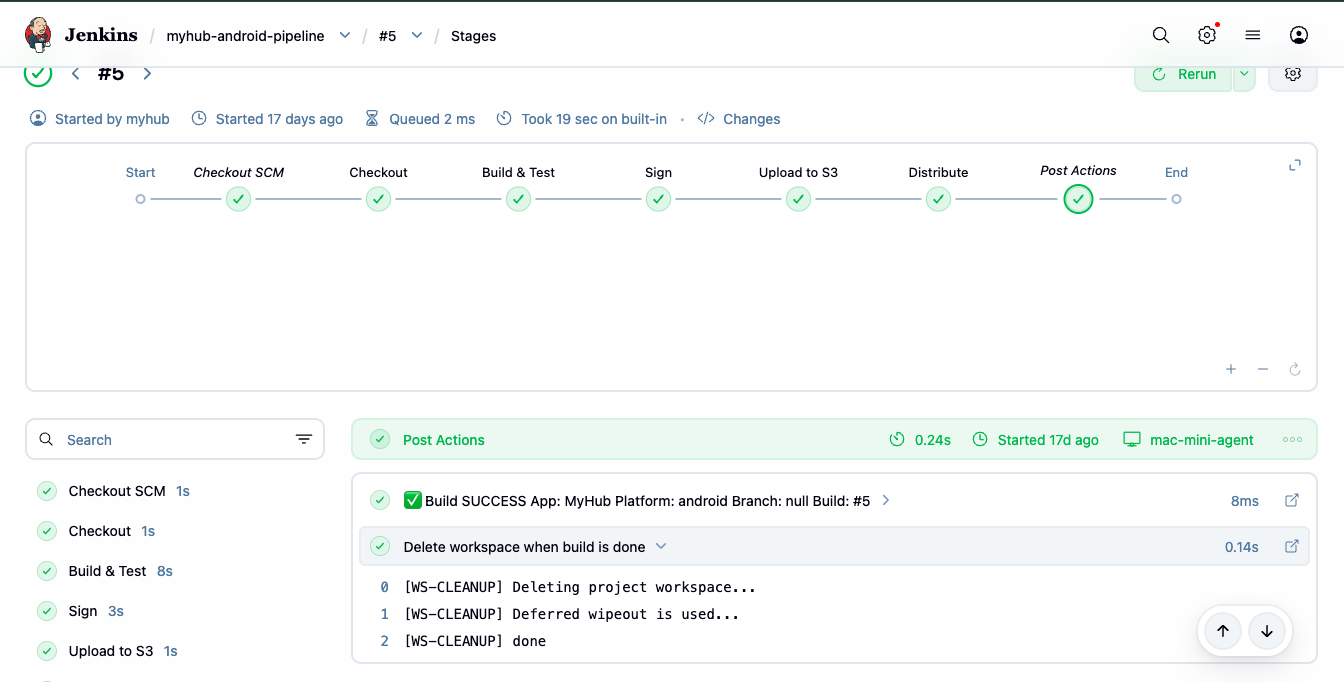
\includegraphics[width=\columnwidth]{figures/jenkins-android-pipeline-success.png}
\caption{End-to-end pipeline runs. Top: iOS build \#17 (total 3\,m\,33\,s).
Bottom: Android build \#5 (total 19\,s). Both complete Checkout, Build \& Test,
Sign, and Upload to S3; Distribute is gated on \texttt{main}.}
\label{fig:pipelines}
\end{figure}

\begin{figure}[t]
\centering
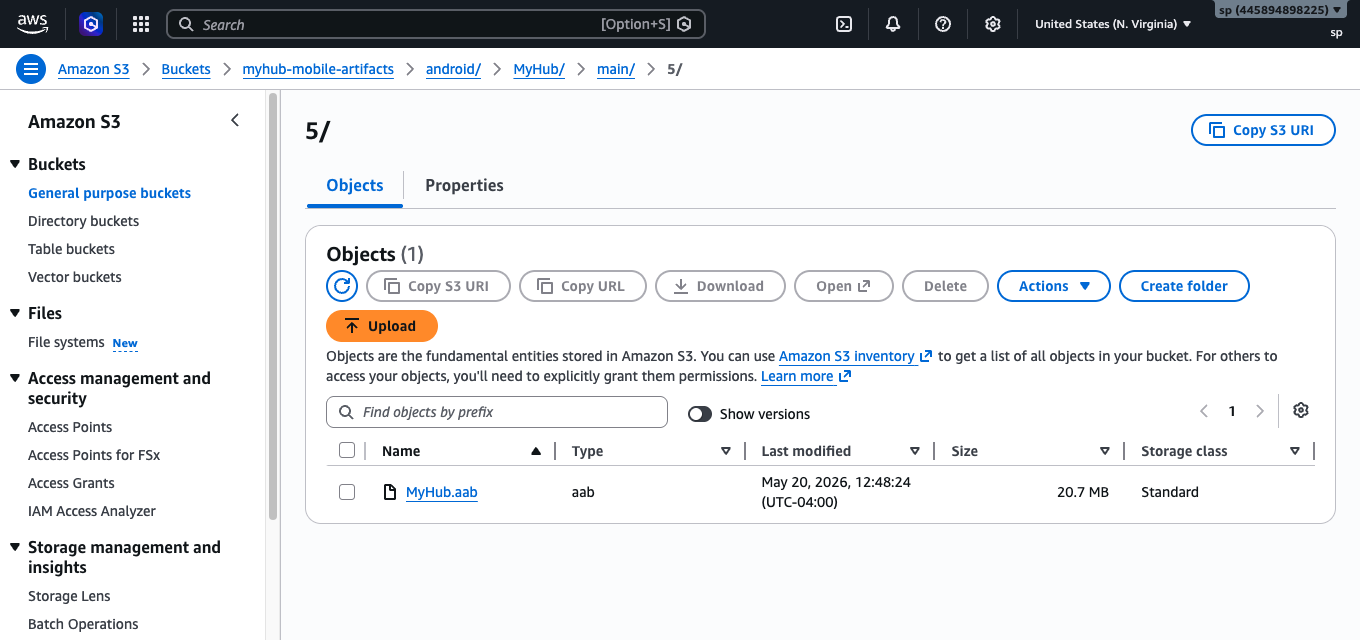
\includegraphics[width=\columnwidth]{figures/s3-android-artifact.png}
\caption{A signed artifact at its versioned key, \texttt{android/MyHub/main/5/},
linking the AAB to the exact build that produced it.}
\label{fig:s3}
\end{figure}

\subsection{Q2: Credential-Exposure Window}
Table~\ref{tab:timings} reports per-stage durations for both runs. The decoded
signing key exists on disk only for the Sign stage: at most 2\,s for the iOS
path and 3\,s for the Android path in these runs. The workspace is then purged.
We contrast this with the persistent-server baseline, in which a copy of the
credential resides on disk continuously. The reduction is qualitative as much as
quantitative: exposure shifts from ``always present, broad blast radius'' to
``present for seconds, scoped to one signing operation.''

\begin{table}[t]
\caption{Per-stage durations (single run per platform).}
\label{tab:timings}
\centering
\footnotesize
\begin{tabular}{@{}lrr@{}}
\toprule
\textbf{Stage} & \textbf{iOS \#17} & \textbf{Android \#5} \\
\midrule
Checkout            & 1\,s        & 1\,s \\
Build \& Test       & 3\,m\,24\,s & 8\,s \\
Sign \emph{(exposure window)} & \textbf{2\,s} & \textbf{3\,s} \\
Upload to S3        & 1\,s        & 1\,s \\
Distribute          & 0.92\,s     & --- \\
Post (notify + purge) & 0.25\,s   & 0.24\,s \\
\midrule
\textbf{Total}      & 3\,m\,33\,s & 19\,s \\
\bottomrule
\end{tabular}
\end{table}

The order-of-magnitude difference in Build \& Test time between platforms
(\texttt{xcodebuild} compiling and running tests on an iOS simulator versus an
incremental Gradle build with a warm cache) is incidental to the security
mechanism; the exposure window is governed by the Sign stage alone and is small
on both platforms.

\subsection{Q3: Onboarding Cost and Monitoring}
Adopting the full pipeline requires the three-line declaration of
Listing~\ref{lst:jenkinsfile} and no other per-application CI code. On the
operability side, the CloudWatch agent forwards three log groups
(\texttt{/jenkins/builds}, \texttt{/jenkins/system},
\texttt{/mac-agents/jenkins-agent}) and a CPU alarm on the build host remained in
the \textsc{ok} state with the agent idle at roughly 4--5\% CPU between builds,
confirming that metrics flow from the private-subnet host to CloudWatch (G7).

%==============================================================================
\section{Discussion}\label{sec:discuss}
%==============================================================================
\subsection{Portability}
Because all pipeline logic resides in the shared library and the only
source-control coupling is a repository URL and a credential identifier,
migrating from GitHub to Bitbucket requires no change to pipeline code---only new
credentials and webhook configuration. Similarly, an enterprise release gate such
as IBM UrbanCode Deploy can be inserted as an additional publish stage without
disturbing the build or signing stages. Both integrations are documented in the
repository.

\subsection{Scalability}
Agents share a Jenkins label and are load-balanced automatically; throughput
scales horizontally by registering additional EC2 Mac hosts under the same label.
We did not load-test this dimension.

\subsection{Limitations and Threats to Validity}\label{sec:limits}
We state these plainly, as they bound our claims:
\begin{itemize}
  \item \textbf{iOS signing is demonstrated by design, not by execution with a
  production certificate.} In our prototype the iOS Sign stage packages a
  simulator build (\texttt{CODE\_SIGNING\_ALLOWED=NO}); the production
  temporary-keychain signing path is implemented as the documented
  \texttt{security}/\texttt{xcodebuild} sequence but was not exercised against a
  paid Apple Developer distribution certificate. The Android path \emph{is}
  fully exercised end to end with a real keystore and \texttt{jarsigner}.
  \item \textbf{Distribution is stubbed.} The Distribute stages contain the
  production Fastlane invocations but no live store upload was performed, as that
  requires paid App Store and Google Play accounts.
  \item \textbf{Measurements are illustrative, not statistical.} Timings are
  single runs of one application on one warm agent; they are not a benchmark and
  we make no head-to-head performance comparison against hosted CI.
  \item \textbf{Single-agent deployment.} Horizontal scaling and controller
  high-availability are designed but unmeasured.
  \item \textbf{No third-party audit or external adoption.} The security
  properties are argued from the design and the observed exposure window; they
  have not been independently audited.
\end{itemize}
Within these bounds, the contribution is the architecture and the
ephemeral-credential pattern, demonstrated end to end for Android and for the
non-signing portions of the iOS pipeline, with the iOS signing path specified in
full.

%==============================================================================
\section{Conclusion}
%==============================================================================
BuildStream is an open-source reference architecture that brings mobile signing
credentials back inside an organization's own AWS account and shrinks their
on-agent lifetime from indefinite to seconds. Its pull--use--destroy pattern,
least-privilege IAM scoping, private-subnet build agents, and Jenkins
shared-library design together provide a secure yet low-friction path to mobile
CI/CD: applications onboard in three lines, and signing credentials are present
on a build host only for the moment a signature is produced. We reported a
working AWS deployment with end-to-end pipeline runs, versioned artifacts, and
monitoring, and we quantified the resulting exposure window while being explicit
about the prototype's limits. The complete implementation and documentation are
publicly available to serve as a reproducible starting point for organizations
that cannot, or will not, surrender custody of their signing keys.

%==============================================================================
\begin{thebibliography}{00}
\bibitem{androidsign} Android Developers, ``Sign your app,'' Google.
\url{https://developer.android.com/studio/publish/app-signing}.
\bibitem{applesign} Apple Inc., ``Code Signing,'' Apple Developer Documentation.
\url{https://developer.apple.com/documentation/security/code-signing-services}.
\bibitem{saltzer} J. H. Saltzer and M. D. Schroeder, ``The protection of
information in computer systems,'' \emph{Proc. IEEE}, vol. 63, no. 9,
pp. 1278--1308, 1975.
\bibitem{awssm} Amazon Web Services, ``AWS Secrets Manager User Guide,'' 2024.
\url{https://docs.aws.amazon.com/secretsmanager/}.
\bibitem{vault} HashiCorp, ``Vault: Secrets management,'' 2024.
\url{https://www.vaultproject.io/}.
\bibitem{nistssdf} M. Souppaya, K. Scarfone, and D. Dodson, ``Secure Software
Development Framework (SSDF) Version 1.1,'' NIST SP 800-218, 2022.
\bibitem{jenkins} Jenkins Project, ``Jenkins User Documentation: Shared
Libraries,'' 2024. \url{https://www.jenkins.io/doc/book/pipeline/shared-libraries/}.
\bibitem{fastlane} Fastlane, ``Fastlane docs,'' 2024.
\url{https://docs.fastlane.tools/}.
\bibitem{ghactions} GitHub, ``GitHub Actions Documentation,'' 2024.
\url{https://docs.github.com/actions}.
\bibitem{ec2mac} Amazon Web Services, ``Amazon EC2 Mac Instances,'' 2024.
\url{https://docs.aws.amazon.com/AWSEC2/latest/UserGuide/ec2-mac-instances.html}.
\end{thebibliography}

\end{document}
